%\documentclass[linenumbers, RNAAS, trackchanges]{aastex631}
\documentclass[linenumbers, twocolumn]{aastex631}

\usepackage[utf8]{inputenc}
\usepackage{hyperref}           % hrefs
\usepackage{natbib}             % for bibliography
\usepackage{float}              % figure positioning
\usepackage{svg}                % used for SVG images
\usepackage{graphicx}           % used for non-SVG images
\usepackage{amsmath}
\usepackage{parskip}


% Search Query Metadata
\shorttitle{Bessel Functions}
%\shortauthors{Nguyen & Sae}

% Hyperlink setup
\hypersetup{
colorlinks=true,
linkcolor=blue,
urlcolor=blue
}

\begin{document}
\title{Numerical Analysis of Bessel Function Roots and their Physical Applications}
% [] is for ORCiD
%\correspondingauthor{Main Author}
%\email{author1@email.com, author2@email.com, author3@email.com}
\author{Lily Nguyen}
\affiliation{Department of Physics, The University of Texas at Austin\\
Austin, TX 78712, USA}

\author{Andre Sae}
\affiliation{Department of Physics, The University of Texas at Austin\\
Austin, TX 78712, USA}


% 250 word limit for abstract
\begin{abstract}

In this project, we numerically computed and visualized the first five positive
roots of the Bessel functions of the first kind, $J_0(x)$, $J_1(x)$, and $J_2(x)$,
using Python. These functions solve a second-order differential equation that 
occur in problems with radial symmetry. We used the \texttt{scipy} library to
evaluate $J_n(x)$ and locate its roots via the \texttt{fsolve} method. We
interpreted the computed roots in the context of three physical materials: the
radial wavefunction in a quantum infinite square well, heat conduction in
cylindrical geometries, and vibrational modes of a circular drumhead. Our
results show how Bessel function roots reflect physical boundary conditions
and demonstrate the usefulness of numerical methods in modeling such systems.

\end{abstract}

% Use astrothesaurus numbers in place of num
\keywords{Bessel functions --- root-finding --- radial symmetry --- boundary value problems --- numerical analysis}


\section{Introduction} \label{sec:intro}

The Bessel functions of the first kind, $J_n(x)$, are solutions to the
second-order linear differential equation:
\begin{equation}
    z^2\frac{d^2 w}{dz^2}+z\frac{dw}{dz}+(z^2-n^2)w=0,
\end{equation}
\noindent where integer $n=0,1,2\dots$ represents the order of the
function. These functions appear naturally in the separation of variables when solving
partial differential equations in cylindrical or spherical coordinates,
particularly in systems with radial symmetry. Bessel functions also have an
integral
\begin{equation}
    J_n(x)=\frac{1}{\pi}\int_0^\pi cos(x\sin\theta-n\theta)d\theta
\end{equation}
\noindent for integers $n=0,1,2\dots$, which is particularly useful for understanding 
their oscillatory behavior.

\noindent Bessel functions were first introduced by German astoronomer and
mathematician Friedrich Wilhelm Bessel in the early 1800s during his study of
planetary orbits. However, the equation itself had been investigated earlier
by Bernoulli and Euler in problems involving vibrational membranes
\citet{abramowitz_stegun}. Today, Bessel functions are foundational tools in 
mathematical physics and engineering. In quantum mechanics, they appear in 
radial solutions to the Schrödinger equation for quantum wells CITE, in the 
vibration modes of circular membranes like drumheads CITE, and in heat 
conduction problems with cylindrical geometries CITE.

\noindent In this project, we numerically compute the first five positive roots
of the Bessel functions $J_0(x)$, $J_1(x)$, and $J_2(x)$. These roots correspond
to physically meaningful quantities such as resonance modes, cutoff frequencies, 
or quantized boundary values in systems with radial symmetry. We use Python to visualize each
function, estimate the approximation locations of their roots, and apply the \texttt{fsolve}
method from \texttt{scipy.optimize} to compute each root with high precision. 
Our goal is to obtain accurate roots values for each order and verify them 
using numerical methods


\section{Data and Observations} \label{sec:data}

This project focuses on computing and visualizing the first five roots of the
Bessel functions of the first kind, $J_n(x)$, for orders $n=0,1,2$. These
functions solve the second-order linear differential equation:
\begin{equation}
    z^2\frac{d^2 w}{dz^2}+z\frac{dw}{dz}+(z^2-n^2)w=0,
\end{equation}
\noindent which arise in physical systems with spherical or cylindrical 
symmetry. The positive roots of $J_n(x)$ represent physically meaningful
quantities such as resonant frequencies or quantized energy levels in such
systems.

\noindent We computed the Bessel functions using Python's \texttt{scipy.special.jv}
method, which evaluates $J_n(x)$ for an arbitrary order and argument. To
find the roots numerically, we used the \texttt{fsolve} method from \texttt{scipy.optimize},
which refines an initial guess until it finds a point where the function crosses
zero. We chose a set of initial guesses based on where the function appeared to
cross the x-axis in the plot and passed those values into \texttt{fsolve} to
calculate each root more precisely. We used the following initial guesses:

\begin{itemize}
    \item $J_0(x)$: [2, 6.1, 8.6, 11.7, 15]
    \item $J_1(x)$: [3.9, 7, 10.15, 13.1, 16.4]
    \item $J_2(x)$: [5.1, 8.3, 11.8, 14.9, 18]
\end{itemize}

\noindent This gave us exactly five positive roots for each Bessel function. The 
resulting plots of $J_0(x)$, $J_1(x)$, and $J_2(x)$ over the domain $x=0$ to
$x=20$ are shown in Figure~\ref{fig:bessel_roots}, with the first five roots of
each function marked as scatter points.

\begin{figure}[H]
    \centering
    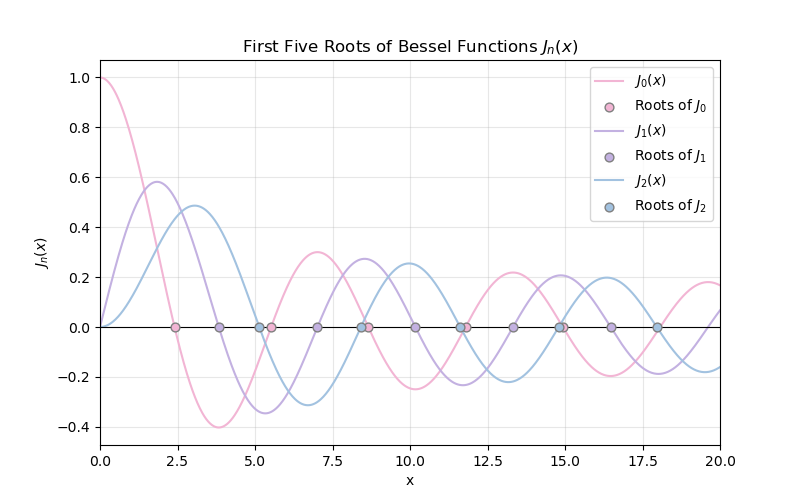
\includegraphics[width=1.0\linewidth]{bessel_roots.png}
    \caption{Bessel functions $J_0(x)$, $J_1(x)$, and $J_2(x)$ plotted from $x=0$ to
    $x=20$, with their first five positive roots represented as circular markers.}
    \label{fig:bessel_roots}
\end{figure}


\section{Results} \label{sec:results}

The plots of $J_0(x)$, $J_1(x)$, and $J_2(x)$ from $x=0$ to $x=20$ show that
Bessel functions of the first kind exhibit oscillatory behavior with gradually
decaying amplitude. As expected, $J_0(x)$ begins at $1$, while higher-order
functions satisfy $J_n(x)=0$. The zero crossings become slightly less
frequent as $x$ increases.

\noindent The computed roots correspond to the first five positive values of $x$
for which $J_n(x)=0$ and are marked as circular points in Figure~\ref{fig:bessel_roots}.
These roots are important in radial problems where boundary conditions require the
function to vanish at a specific radius. For example, they determine the allowed
energy levels in circular quantum wells, resonance frequencies in drumhead 
vibrations, and decay rates of thermal modes in cylindrical heat conduction.

\noindent Our numerical results followed the expected trend that root values
increase with both the order $n$ and the root index. This quantized structure
highlights the physical significance of Bessel function solutions in bounded
radial domains.


\section{Applications} \label{sec:applications}

ADD IN CITATIONS AND REORGANIZE THIS SECTION\\

Bessel functions arise naturally in the solutions to a wide variety of physical
problems that exhibit radial symmetry. In this section, we highlight three
examples: the infinite square well in quantum mechanics, radial thermal
diffusion, and wave propagation on a circular membrane. In each case, Bessel
functions emerge from imposing boundary conditions on the radial part of a 
separable partial differential equation.

\subsection{Quantum Mechanics: The Infinite Square Well}

Bessel functions appear in the solution to the Schrödinger equation for a
particle confined in a three-dimensinoal infinite spherical potential well.
The potential is defined as:

\begin{equation}
    V(x)=
    \begin{cases}
        0, &\text{if }r < a\\
        \infty, &\text{if }r\geq a
    \end{cases}
\end{equation}

The time-independent radial Schrödinger equation in spherical coordinates becomes:
\begin{equation}
    \hat{H}\psi-E\psi=\hat{H}R_{n,l}-ER_{n,l}=0
\end{equation}
\begin{equation}
    \hat{H}=\frac{-\hbar ^2}{2m}\left(\frac{\partial^2}{\partial r^2} + \frac{2}{r} \frac{\partial}{\partial r} - \frac{l(l+1)}{r^2}\right) +V(r)
\end{equation}
\noindent where $\hat{H}$ is the Hamiltonian operator and $E$ is the energy eigenvalue.

\noindent Inside the well ($r<a$), the radial equation reduces to:
\begin{equation}
    r^2\frac{\partial^2 R_{n,l}}{\partial r^2} + 2r\frac{\partial R_{n,l}}{\partial r} +(k^2r^2-l(l+1))R_{n,l}=0
\end{equation}

\noindent This is recognizeed as the spherical Bessel differential equation.
Its solutions are the spherical Bessel functions $j_l(k_{n,l},r)$, which are related
to the ordinary Bessel functions by:
\begin{equation}
    j_l(k_{n,l},r)=\sqrt{\frac{\pi}{2kr}}J_{l+\frac{1}{2}}(k_{n,l}r)
\end{equation}

\noindent Imposing the boundary condition $j_l(ka)=0$ leads to discrete values $k_{n,l}$,
which quantize the energy levels as:
\begin{equation}
    E_{n,l}=\frac{\hbar^2k_{n,l}^2}{2ma^2}
\end{equation}

Thus, the Bessel function roots determine the allowed energy states of the system.


------------------------------------------------------------------------

The Hamiltonian operator $\hat{H}$ and energy operator $\hat{E}$ must also be
defined to compute the wavefunction. The $n$ and $i$ are quantum numbers where $n$
is the principle quantum number and $I$ is the angular momentum quantum number where
both span the integer range from zero to infinity. $\hbar$ is Planck's constant, $m$
is the mass of the particle, $r$ is the radius, and $R_{n,l}$ is the wavefunction in
the radial basis.

\begin{equation}
    \hat{H}=\frac{-\hbar ^2}{2m}\left(\frac{\partial^2}{\partial r^2} + \frac{2}{r} \frac{\partial}{\partial r} - \frac{l(l+1)}{r^2}\right) +V(r)
\end{equation}

\begin{equation}
    \hat{H}\psi-E\psi=\hat{H}R_{n,l}-ER_{n,l}=0
\end{equation}

\noindent Applying the Hamiltonial operator on the wavefunction gives us the
spherical Bessel function in differential form, which looks similar to the
origianl Bessel function in differential form:

\begin{equation}
    r^2\frac{\partial R_{n,l}}{\partial r^2} + 2r\frac{\partial R_{n,l}}{\partial r} +(k^2r^2-l(l+1))R_{n,l}=0
\end{equation}

\noindent To obtain a solution, we impose a boundary condition $j_l(k_{n,l}a)=0$ at the
bounds of the well. This quantizes our solution by setting a discrete energy
level $E_{n,l}=\frac{\hbar^2k_{n,l}^2}{2ma^2}$ where the solution exists. Hence,
we are left with a radial solution to the wave equation containing the original
Bessel Function:

\begin{equation}
    R_{n,l}=Aj_l(k_{n,l}r)
\end{equation}

\noindent where $j_l(k_{n,l},r)=\sqrt{\frac{\pi}{2kr}}J_{l+\frac{1}{2}}(k_{n,l}r)$.\\


\subsection{Thermal Diffusion}

Bessel functions also arise in radial heat conduction problems. The temperature
distribution $T(r,t)$ in a two-dimensional circular region is governed by the
heat equation:
\begin{align}
    \frac{\partial T}{\partial t}&=\alpha\nabla^2T\\
    &=\alpha\left(\frac{1}{r} \frac{\partial T}{\partial r} + \frac{\partial^2 T}{\partial r^2}\right)
\end{align}
\noindent where $\alpha=\frac{k}{\rho c_p}$.

\noindent Using separation of variables with $T(r,t)=X(r)\theta(t)$, the spatial equation becomes:
\begin{equation}
    \frac{d^2X}{dr^2}+\frac{1}{r}\frac{X}{r}+\lambda^2X=0.
\end{equation}

\noindent THis is the Bessel equation of order zero. Solutions involve the
Bessel function $J_0(\lambda r)$, and applying the boundary condition 
$T(r,t)=T_1$ leads to quantization in terms of the roots $\beta_n$ such
that $J_0(\beta_0)=0$.

\noindent The full solution is:

REWRITE/SIMPLIFY EQN TMRW

\noindent The decay of each mode over time depends on the root $\beta_n$,
which emphasizes how Bessel zeroes influence the thermal dynamics of
circular geometries.


------------------------------------------------------------------------

We define the heat equation propagating through a two-dimensional surface in
the radial direction. $T$ is the temperature, $t$ is the time, $r$ is the radius,
$k$ is the material conductivity, $\rho$ is the density of the material, and $c_p$
is the specific heat capacity.

\begin{align}
    \frac{\partial T}{\partial t}&=\alpha\nabla^2T\\
    &=\alpha\left(\frac{1}{r} \frac{\partial T}{\partial r} + \frac{\partial^2 T}{\partial r^2}\right)
\end{align}

\noindent where $\alpha=\frac{k}{\rho c_p}$.

To solve this equation, we use separation of variables to split the 
differential equation into two separate differential equations and assume
that one takes the form $T(r,t)=X(r)\theta(t)$. The first equation takes the
form of exponential decay over time:

\begin{equation}
    \frac{d\theta}{dt}+\lambda^2\alpha\theta=0
\end{equation}

\noindent whereas the second equation is the Bessel function of the zeroth-order
since $\alpha=0$:

\begin{equation}
    \frac{d^2X}{dr^2}+\frac{1}{r}\frac{X}{r}+\lambda^2X=0.
\end{equation}

We set a boundary condition of $T(r,t)=T_1$, where $R$ is the radius of the circle,
$t$ is time with $t>0$, and $T_1$ is a constant real value. The initial condition for
the radial space is defined as $T(r,0)=T_2$, where $T_2$ is a constant real value.

\begin{equation}
    T^*=\frac{T(r,t)-T(R,t)}{T(r,0)-T(R,t)}=2\sum_{n=0}^\infty e^{-\beta_{n}^2 \frac{\alpha t}{R^2}} \frac{J_0(\beta_n\frac{r}{R})}{\beta_nJ_1(\beta_n)}
    \label{eq:T_star}
\end{equation}

\begin{equation}
    T(r,t)=T^*(T(r,0)-T(R,t))+T(R,t)
    \label{eq:T}
\end{equation}

\noindent We define temperature as a unitless quantity $T^*$. $\beta_n$ is the
nth-root solution where $J_0(r)=0$. The temperature function uses both the zeroth
and first order Bessel function in the solution. Hence, Equation~\ref{eq:T_star}
and Equation ~\ref{eq:T} is the final solution for that the temperature takes.\\


\subsection{Drum Wave Propagation}

The vibration of a circular membrane, such as a drumhead, is another problem
where Bessel functions appear. The vertical displacement $z(r,\theta,t)$
satisfies the two-dimensional wave equation:
\begin{equation}
    \frac{\partial^2z}{\partial t^2}=c^2\nabla^2z
\end{equation}
\noindent where $c^2=\frac{\sigma^2}{S}$.

\noindent Assuming axisymmetric vibrations and separating variables, we arrive
at the radial equation:
\begin{equation}
    r^2\frac{\partial^2R}{\partial r^2}+r\frac{\partial R}{\partial r}+(\lambda^2r^2-n^2)R=0
\end{equation}

\noindent whose solutions are $J_m(\lambda r)$. The boundary condition $(R_f)=0$
implies that $\lambda$ must be a root $\lambda_{m,k}$ of the Bessel function
$J_m(\lambda r)$. Thus, the full solution becomes:

REWRITE/SIMPLLIFY EQN TMRW


\noindent These roots define the resonance frequencies of the drumhead and
determine its modes of vibration.


------------------------------------------------------------------------

Drum wave propagation is similar to thermal diffusion regarding classical wave 
mechanics and quantum mechanics through the quantization of boundary conditions.
We define a wavefunction for the propagation across a drum surface where $\sigma$
is the surface mass density of the membrane and $S$ is the surface tension
across the membrane:

\begin{equation}
    \frac{\partial^2z}{\partial t^2}=c^2\nabla^2z
\end{equation}

\noindent where $c^2=\frac{\sigma^2}{S}$.

\noindent The first boundary condition is $z(R_f,t)=0$. The displacement from the origin
along the z-axis must be zero at the edge of the drum since those points are
fixed. This condition quantizes the solution, yielding discrete Bessel functions
that satisfy the boundary conditions. To simplify the example, we impose the boundary
condition $z(r,\theta,0)=f(r)$ for $0\leq r \leq a$, representing the initial
pertubation caused by striking the surface at its center. This approach preserves
the $\theta$-dependence in the solution, allowing the Bessel function to appear
explicitly in the radial component.

\begin{equation}
    z(r,\theta,t)=R(r)T(t)\Theta(\theta)=R(r)T(t)
\end{equation}

\begin{equation}
    r^2\frac{\partial^2R}{\partial r^2}+r\frac{\partial R}{\partial r}+(\lambda^2r^2-n^2)R=0
\end{equation}

\begin{equation}
    \frac{dT}{dt}+\lambda^2cT=0
\end{equation}

\begin{eqnarray}
    n=\lambda_{m,k}
\end{eqnarray}

\begin{eqnarray}
    z(r,t)=\sum_{m=0}^\infty \sum_{k=1}^\infty J_m(\lambda_{m,k}r)e^{-c\lambda_{m,n}t}
\end{eqnarray}

\noindent Finally, impose a boundary condition enforcing zero displacement at
the drum's boundary:

\begin{equation}
    J_m(\lambda_{m,k}R_f)=0,
\end{equation}

\noindent where $m$ is the order of the Bessel function and $k$ is the wavenumber.
For $m=0$, the Bessel function itself vanishes at the boundary. There exist infinitely
many integer values of $m$ and $k$ for which this condition is satisfied, corresponding
to the distinct vibration modes of the drumhead. The resulting function $z(r,t)$
describes the final waveform of the drum's vibration in time.


\section{Summary and Conclusion} \label{sec:summary}

In this project, we explored the roots of the Bessel functions of the first kind, 
$J_n(x)$, for orders $n=0,1,2$ using Python's \texttt{scipy} library. Our numerical
approach combined the built-in evaluation of $J_n(x)$ with the \texttt{fsolve}
method to accurately identify the first five positive roots for each order. Our
results aligned well with the expected theoretical behavior, including the trends
in oscillation decay and root spacing.

\noindent The numerical methods we used were sufficiently accurate for our goals.
Plotting the functions alongside their roots helped us visualize their role in
physical boundary value problems with radial symmetry. While the method was
effective, it relied on manually chosen initial guesses. This could be improved in
future work by using analytical approximations or implementing a more automated
root-finding strategy.

\noindent Overall, this project demonstrated how Bessel functions can be approached
computationally, how their oscillatory behavior varies with order, and why their
roots are important physical systems. Further work could involve exploring other 
families of Bessel functions or extending the root-finding method to more
advanced applications involving partial differential equations where these functions
naturally arise due to symmetry. These additions would provide deeper insight into the
mathematical structure and wide-ranging applications of Bessel functions.


\subsection{Acknowledgements}
We thank Professor Mitra for his guidance and instruction throughout the course,
as well as the teaching assistants for their helpful feedback. We also
acknowledge the Department of Physics for providing an excellent academic foundation 
to support this work. This work was completed as part of the requirements for 
C S 323E: Elements of Scientific Computing at the University of Texas at Austin.

\newpage
\bibliographystyle{aasjournal}
\bibliography{refs}

\end{document}